%! alt Equilateral triangle ABE drawn dashed, with D on side AE and C on side BE. The quadrilateral ABCD has 60 degree angles at A and B; the shaded triangle DEC that is cut off has a 60 degree angle at E, with ED = x and EC = y. In the case drawn AB = 12, x = 3, y = 8 and CD = 7.
%! after_paragraph 1
%! scale 2/3
% The shared preamble of every Cevian figure. pipeline/figures turns these colours into theme-aware paint,
% and refuses any other colour, so draw only with them:
%   figink (lines and labels), figaux (construction lines), figaccent (the object the argument turns on),
%   figtint and figaccenttint (light fills).
\documentclass[border=1.5pt]{standalone}
\usepackage{tkz-euclide}
\definecolor{figink}{RGB}{0,0,0}
\definecolor{figaux}{RGB}{85,85,85}
\definecolor{figaccent}{RGB}{192,57,43}
\definecolor{figtint}{RGB}{221,221,221}
\definecolor{figaccenttint}{RGB}{245,213,208}
% tkz-euclide's defaults draw circles, compasses and marks in 50% grey and fill points with a tint.
\makeatletter
\def\tkz@otherlinecolor{figink}
\def\tkz@euc@circlecolor{figink}
\def\tkz@euc@compasscolor{figink}
\def\tkz@euc@mkcolor{figink}
\def\tkz@mk@fill{figink}
\def\tkz@euc@pointfillcolor{figink}
\makeatother
\tkzSetUpLine[color=figink,line width=.7pt]
\tkzSetUpArc[color=figink,line width=.7pt]
\tkzSetUpCompass[color=figink,line width=.5pt]
\tkzSetUpPoint[color=figink,fill=figink,size=3.1pt]
\tikzset{
  every picture/.style={line cap=round,line join=round,color=figink},
  circle style/.append style={color=figink,line width=.7pt},
  aux/.style={color=figaux,line width=.45pt,dash pattern=on 2.6pt off 2pt},
  key/.style={color=figaccent,line width=1pt},
  mk/.style={color=figink,line width=.5pt},
  lbl/.style={color=figink,inner sep=2.2pt},
  len/.style={color=figink,inner sep=1.5pt,font=\small},
}

\begin{document}
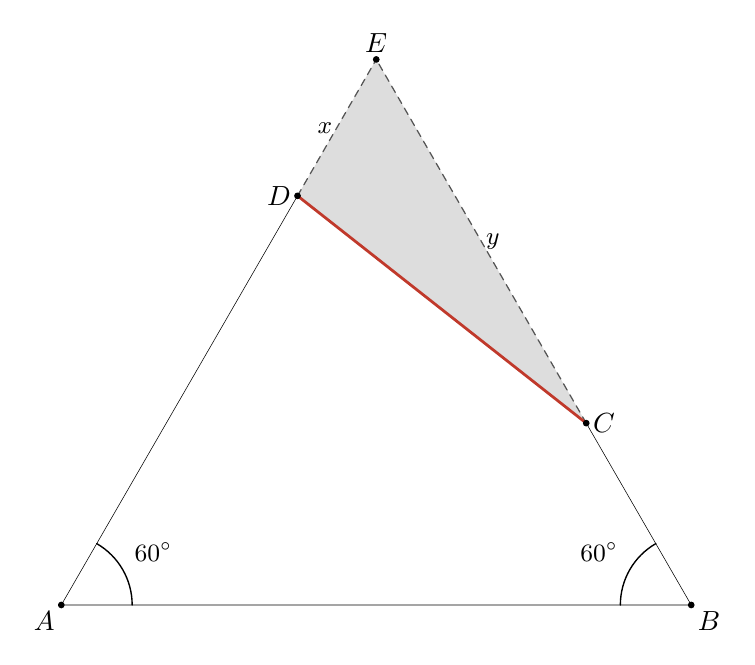
\begin{tikzpicture}
\tkzDefPoint(0.0,0.0){A} %! A = (0, 0)
\tkzDefPoint(8.0000000,0.0){B} %! B = (12, 0)
\tkzDefPoint(4.0000000,6.9282032){E} %! E = (6, 6*sqrt(3))
\tkzDefPoint(3.0000000,5.1961524){D} %! D = (9/2, 9*sqrt(3)/2)
\tkzDefPoint(6.6666667,2.3094011){C} %! C = (10, 2*sqrt(3))
%! fact angle(D, A, B) == 60
%! fact angle(A, B, C) == 60
%! fact angle(D, E, C) == 60
%! fact collinear(D, A, E)
%! fact collinear(C, B, E)
%! fact dist(C, D)**2 == dist(E, D)**2 - dist(E, D) * dist(E, C) + dist(E, C)**2
%! example dist(A, B) == 12
%! example dist(E, D) == 3
%! example dist(E, C) == 8
%! example dist(C, D) == 7
\tkzFillPolygon[color=figtint](D,E,C)
\tkzDrawSegment[aux](D,E)
\tkzDrawSegment[aux](C,E)
\tkzDrawPolygon(A,B,C,D)
\tkzDrawSegment[key](C,D)
\tkzMarkAngle[size=.9,arc=l,mark=none,mk](B,A,D)
\tkzMarkAngle[size=.9,arc=l,mark=none,mk](C,B,A)
\tkzLabelAngle[pos=1.35,font=\small](B,A,D){$60^\circ$}
\tkzLabelAngle[pos=1.35,font=\small](C,B,A){$60^\circ$}
\tkzDrawPoints(A,B,C,D,E)
\tkzLabelPoint[below left,lbl](A){$A$}
\tkzLabelPoint[below right,lbl](B){$B$}
\tkzLabelPoint[right,lbl](C){$C$}
\tkzLabelPoint[left,lbl](D){$D$}
\tkzLabelPoint[above,lbl](E){$E$}
\tkzLabelSegment[left,len](D,E){$x$}
\tkzLabelSegment[right,len](E,C){$y$}
\end{tikzpicture}
\end{document}
